% The original template (from Trevor) had a custom \appendix command,
% but I found it to break figure/table counters. I'm not sure how
% reliable my fix is, so I ended up reverting back to the standard
% latex version, and renaming the custom command to \myappendix.  You
% can try both and see how things work out:
% 1) Call \appendix once, and then make each appendix a \chapter
% 2) Call \myappendix once, and then make each appendix a \section.

\appendix

\chapter{Ontologie de contexte}

\section{Entités de l'ontologie}

\begin{itemize}
  \item \textbf{Machine} est n'importe quel périphérique en mesure d'accepter et
	  de traiter des informations pour fournir le résultat désiré basé sur
	  un programme ou une séquence d'instructions sur comment les données
	  doivent être traitées.
  \item \textbf{Computers} sont le type principal de machines dans cette étude.
	  C'est pourquoi les deux terminologies sont interchangeables dans
	  diverses sections de ces travaux. Les ordinateurs personnels (PCs),
	  les ordinateurs portables et les serveurs héritent tous de ce type.
  \item \textbf{Operating System} est un programme faisant le pont en les
	  composants logiciels et les composants matériels sous-jacents d'une
	  machine. Le système d'exploitation est une entité comportant plusieurs
	  sous-classes disjointes telles que Windows XP, OS X ou Linux.
  \item \textbf{Packages} sont les programmes applicatifs conçus pour servir un
	  but spécifique comme distribuer un service local, réseau ou web sur
	  une ou plusieurs machines. Le paquet Apache est en bon exemple
	  d'entité conçue pour activer un service web.
  \item \textbf{Service} est une fonctionnalité spécifique d'un système
	  informatique comme un service web ou réseau offert par une machine. Un
	  processus qui est défini dans ce document comme un ensemble ou d'une
	  partie d'un ensemble de mesures permettant la fourniture de services
	  en exécutant des activités réelles en tâche de fond.
  \item \textbf{Command} est un utilitaire pouvant être utilisé par les
	  utilisateurs pour démarrer un processus spécifique, à la condition
	  qu'il n'existe pas de planification pour l'exécution de cette même
	  tâche. Un très bon exemple permettant d'illustrer cette relation
	  entre ces deux entités serait un web service, qui nécessite qu'un
	  processus tel que ''httpd'' soit démarré en arrière plan à l'aide de
	  la commande ''\begin{verbatim}httpd start\end{verbatim}''.
  \item \textbf{Storage} est une partition logique d'un média de stockage
	  physique qui sert principalement d'hôte pour les différents types de
	  fichiers. Un fichier est défini comme une collection d'informations
	  complète comme un programme, un ensemble de données utilisées par un
	  programme ou un document créé par un utilisateur.
  \item \textbf{Interface} est défini comme un périphérique permettant l'accès à
	  un réseau par une machine.
\end{itemize}

\section{Propriétés objets de l'ontologie (Relations)}

\begin{itemize}
  \item \textbf{Caused By} :
          Un type d'association où une entité joue le rôle d'affecter l'autre en
	  changeant son état de l'état X à l'état Y.
  \item \textbf{Configured By} : 
	  Quand une entité X peux apporter les changements nécessaires à
	  l'entité Y pour lui permettre d'accomplir ses objectifs et ses
	  intentions. Le lien entre une machine et un progiciel de gestion de
	  configuration comme CfEngine 3 est un exemple typique de ce type de
	  relations.
  \item \textbf{Edited By} : 
	  Décrit qu'un fichier peut être modifié par un éditeur tel que
	  l'utilisateur du fichier à certaines fins.
  \item \textbf{Managed By} : 
	  Si X est responsable du bon fonctionnement de Y dans l'accomplissement
	  de son objectif, X est dit manager de Y. Le fait qu'une entité hérite
	  de ce rôle implique une supervision constante et des prises de mesures
	  lorsqu'intervient une déviation dans le comportement souhaité.
  \item \textbf{Monitoring By} : 
	  La supervision est principalement la responsabilité de garder un œil
	  sur quelque chose. Si une entité X supervise Y, elle surveille une
	  quelconque altération de comportement pour en informer le ou les
	  managers en charge de cette entité.
  \item \textbf{Component Of} : 
	  La relation entre une entité X, composant d'une entité plus globale Y
      qui joue le rôle d'encapsuleur pour ce composant X.
  \item \textbf{Owned By} : 
	  La propriété est un type de relation pouvant exister entre entité
	  devenue possession et son propriétaire. Le lien entre un fichier et son
	  propriétaire est un exemple de cet type d'association.
  \item \textbf{Promised By} : 
	  La relation en une promesse et l'entité qui la formule. 
  \item \textbf{Required By} : 
	  Si X dépend de Y dans l'accomplissement de ses intentions, la relation
	  entre ces deux entités est de type ''Required By''.
  \item \textbf{Runs On} : 
	  Si l'entité X exerce ses activités ou son exécution sur l'entité Y, la
	  relation est appelé ''Runs On''.
  \item \textbf{Written By} : 
	  La relation entre une écriture X et son auteur Y.
  \item \textbf{Used By} : 
	  Si une entité X fait l'usage d'une entité Y à n'importe quelle moment
	  de son exercice, la relation est de type ''Used By''.
  \item \textbf{Started By} : 
	  Quand une entité X est responsable du démarrage d'une entité Y ou
	  qu'elle commence à se comporter d'un certaine manière, l'association
	  est dite de type ''Started By''.
  \item \textbf{Provided By} : 
	  Quand une entité X a le potentiel et la bonne volonté de fournir
	  quelque chose à une autre entité Y, la relation entre ces deux entités
	  est appelée ''Provided By''.
  \item \textbf{Installed By} : 
	  Une entité X peut mettre en place un programme Y dans une machine de
	  manière à accomplir son but recherché. La relation existante entre X
	  et Y est alors de type ''Installed By''.
  \item \textbf{Contained In} :
	  Si une entité X est contenue dans Y, physiquement ou conceptuellement,
	  la relation est de type ''Contained In''.
\end{itemize}

\section{Propriétés de données de l'ontologie (Attributs)}

\begin{itemize}
  \item \textbf{AllowConnectFrom} : Liste d'adresses IP ou de nom d'hôtes
	  susceptibles d'avoir plus d'une connexion au port d'un serveur.
  \item \textbf{CheckForeign} : Indique s'il est nécessaire de vérifier les
	  autorisations sur le répertoire racine lors de la recherche de la
	  profondeur.
  \item \textbf{CheckRoot} : Liste de nom d'hôtes ou d'adresses IP auxquels
	  accorder un droit de lecture sur le serveur.
  \item \textbf{ForceIpv4} : Indique s'il y a un usage forcé de l'adresse IP
	  pour les connexions.
  \item \textbf{IsMachineVirtualized} : Indique si une machine est virtuelle ou
	  non.
  \item \textbf{PackageFileRepository} : Liste de répertoires locaux à la
	  machine pour la recherche de paquets.
  \item \textbf{TrustKeyFrom} : liste des hôtes pour lesquelles une machine
	  acceptera les clés publiques sur base de la confiance. Définition des
	  types d'occurrences qui sont liés avec le type d'entité stockage sont
	  répertoriés ci-dessous. Un stockage est une partition logique d'un
	  support de stockage physique.
  \item \textbf{FreeSpace} : Pourcentage minimum ou absolu d'espace disque
	  devant être disponible sur le support de stockage avec de lever un
	  avertissement.
  \item \textbf{MountType} : Type de protocole d'un système de fichier distant. 
  \item \textbf{FileSystemFlag} : Liste des options de menu à définir pour les
	  drapeaux de système de fichiers BSD. 
  \item \textbf{Atime} : Plage temporelle d'accès pour les fichiers
	  admissibles.
  \item \textbf{SecureInput} : Indique si les fichiers d'entrée sont accessibles
	  en écriture pour les utilisateurs non-autorisés.
  \item \textbf{MountType} : L'option de menu pour le type de liens à utiliser
	  lors de la copie comme le lien symbolique et le lien physique.
  \item \textbf{AuditingEnabled} : Indique si la fonctionnalité de journal
	  d'audit d'un paquet est activé ou non.
  \item \textbf{LogLevel} : Le niveau de rapport envoyé à syslog.
  \item \textbf{Architecture} : L'architecture relative à la section de paquets
	  comme ''x86-64'' ou ''i386''.
  \item \textbf{BuildsOn} : Liste de groupement de promesses sur lesquelles
	  s'appuie ou dépend une promesse d'une certaine manière (pour la
	  gestion des connaissances)
  \item \textbf{HomeDirectory} : Répertoire contenant les fichiers personnels
	  d'un utilisateur.
  \item \textbf{ShellAccount} : Compte personnel donnant accès à une invite de
	  commande Unix.
  \item \textbf{Module} : Indique s'il faut s'attendre à un protocole de module
	  CfEngine.
\end{itemize}

\chapter{Interface d'administration}

\begin{figure}[H]
    \centerline{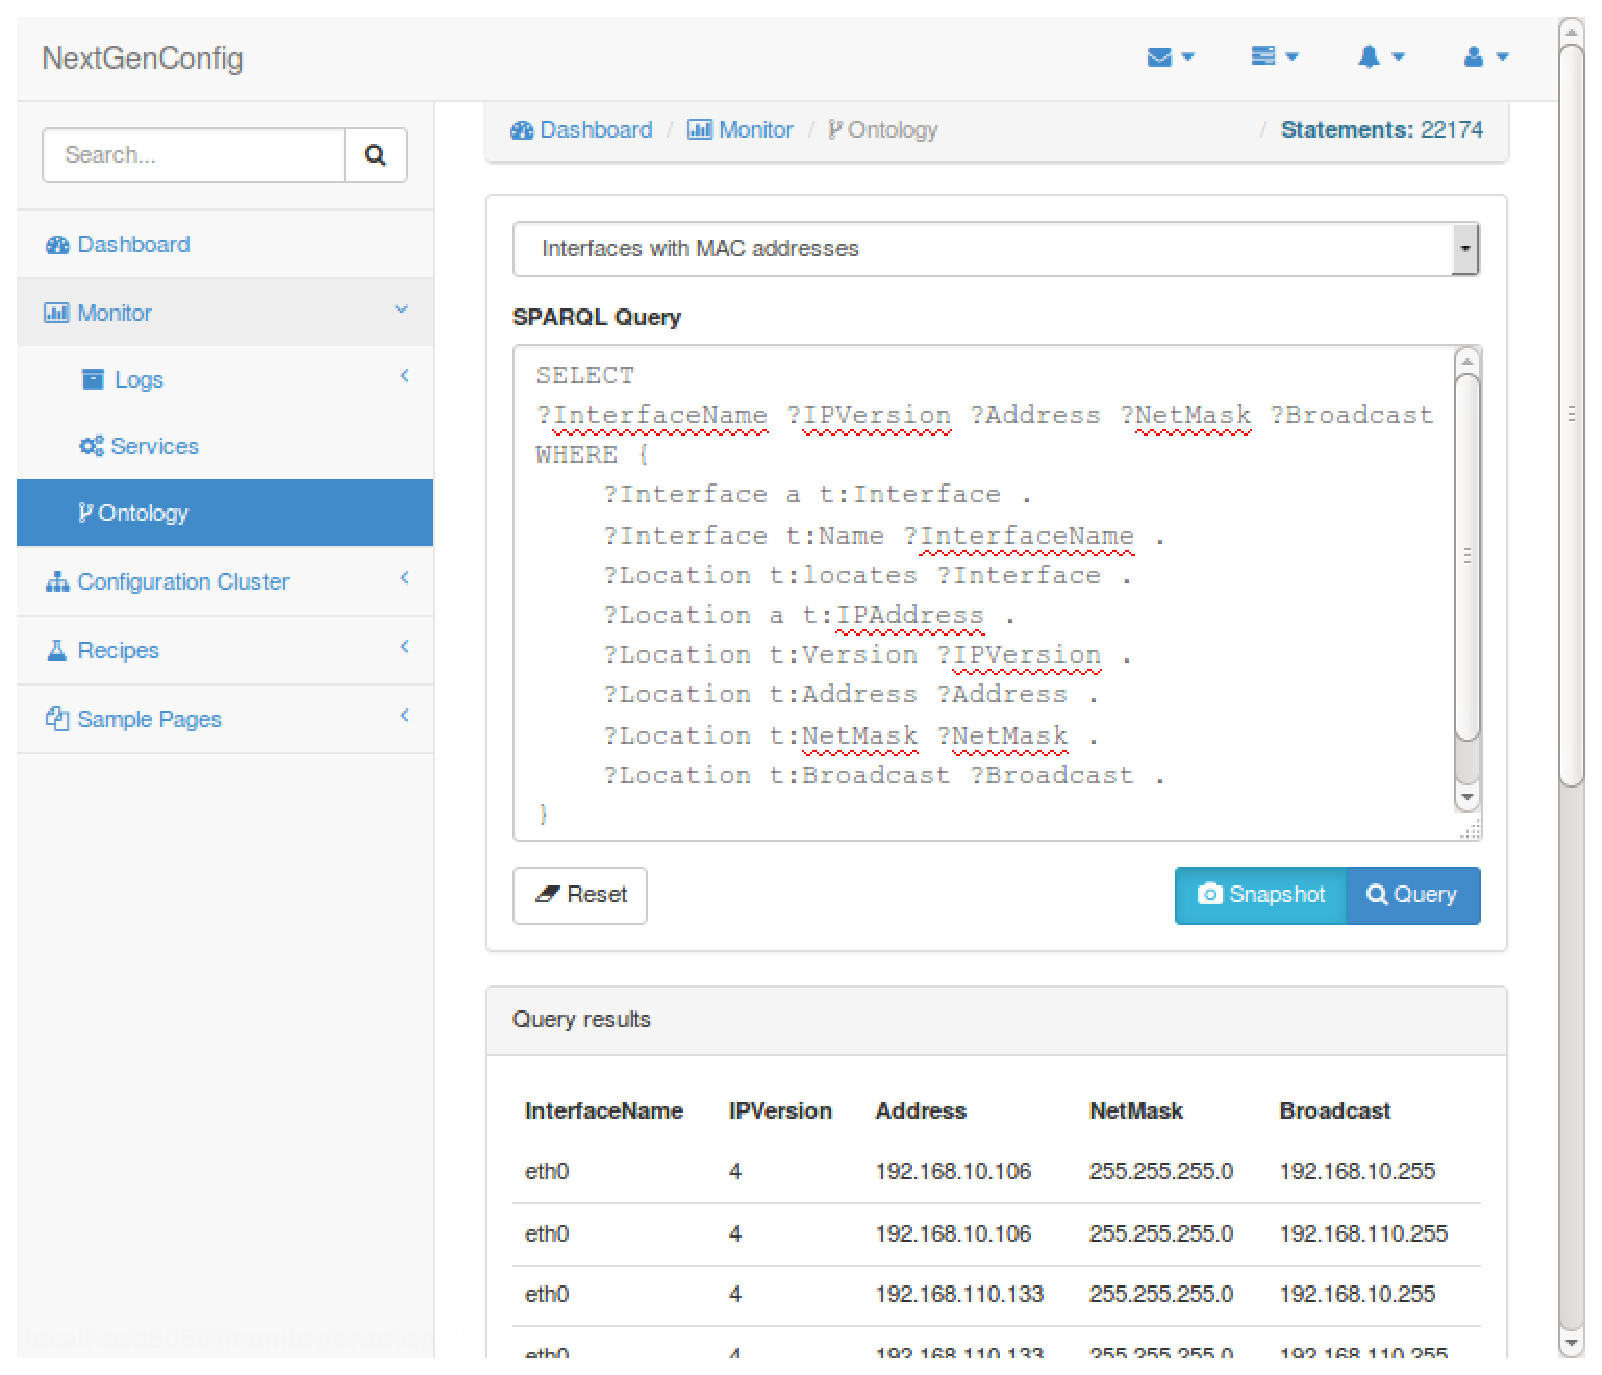
\includegraphics[width=\textwidth]{img/trifle_gui}}
    \caption{Interface d'administration du gestionnaire de configuration}
    \label{fig:trifle_gui}
\end{figure}

% ex: set spelllang=fr spell: %
%%% Local Variables: ***
%%% mode: latex ***
%%% TeX-master: "thesis.tex" ***
%%% End: ***
